% Krishi Mitra -- 6-page IEEE conference paper.
% Section structure follows the guide's outline (report/DocScanner ... .pdf, page 3).
% Compile with pdfLaTeX on Overleaf. Red TODO text = author names and affiliation to fill in.
\documentclass[conference]{IEEEtran}
\usepackage{url}
\usepackage{amsmath,amssymb}
\usepackage{graphicx}
\usepackage{booktabs}
\usepackage{xcolor}
\usepackage{cite}
\usepackage{tikz}
\usetikzlibrary{arrows.meta,positioning}
\newcommand{\todo}[1]{\textcolor{red}{\textbf{[TODO: #1]}}}

\begin{document}

\title{Refuse Rather Than Guess: A Safety-First Kannada Question-Answering Assistant for Sugarcane Farmers}

\author{\IEEEauthorblockN{\todo{Author names}}
\IEEEauthorblockA{\todo{Department, college, city, India}\\
\todo{emails}}}

\maketitle

\begin{abstract}
A wrong pesticide or dose can destroy a crop or harm the person spraying it, so an
agricultural assistant must be judged first on whether it ever gives a wrong
recommendation. We report building a Kannada question-answering assistant for sugarcane
farmers in Karnataka in two versions. Version~1 is a retrieval-augmented generation (RAG)
pipeline with BGE-M3 hybrid retrieval, an abstention gate, and two answer checks (an LLM
faithfulness judge and a rule-based numeric check). We describe safety failures found while
building it, including a gate that read a rank-based fusion score and judge and router calls
that failed silently, and show that ROUGE-L scores 6 of 16 Kannada references 0.000 against
themselves, while chrF and BLEU score a 10$\times$ overdose (96.7 chrF) above a correct
paraphrase (62.5). On 40 held-out questions, version~1 made 29 correct answer-or-refuse
decisions but gave one dose for the wrong pest, which both answer checks rated faithful.
Version~2 removes the language model from the answer path: questions are matched
deterministically to typed fact records drafted from two university Packages of Practices,
and only records a person has confirmed against the printed page are shown.
With 50 of 90 records confirmed and their pesticides cross-checked against the national
registration list, two pilots with 30 new questions gave 27 correct decisions, all 13
should-refuse questions refused, and no wrong dose; all three errors were refusals.
\end{abstract}

\begin{IEEEkeywords}
agricultural advisory, retrieval-augmented generation, Kannada, abstention, evaluation, safety
\end{IEEEkeywords}

% =========================================================
\section{Introduction}
Karnataka is India's third-largest sugarcane producer: 48.06 million tonnes from 0.54 million
hectares in 2024--25, about 10.6\% of national production~\cite{pib2025sugarcane}. Over a
season of a year or more the farmer chooses a variety, treats setts, applies fertiliser in
splits and controls pests and diseases, and the official recommendations differ between
southern Karnataka (UAS Bengaluru) and northern Karnataka (UAS Dharwad). These
recommendations are in long printed books; extension staff are few; and most farmers ask
in Kannada.

\textbf{Traditional approach.} Farmers rely on extension officers, input dealers and the
Kisan Call Centre (KCC, 1800-180-1551), which gives expert answers in local languages but
depends on call-centre capacity.

\textbf{Existing AI approaches.} Recent agricultural assistants use large language models
(LLMs) with retrieval-augmented generation (RAG)~\cite{lewis2020rag,vijayvargia2025krishisathi,singh2024farmerchat,samuel2025agrollm}.
They are usually evaluated on accuracy over answerable questions, answer similarity, or
LLM-judged quality. In this domain, however, the
costly error is a fluent answer with a wrong chemical, dose or unit, and similarity metrics
do not detect it (Section~\ref{sec:results}).

\textbf{Contributions.} (1) A Kannada RAG pipeline for sugarcane and the safety failures
found and fixed in it; (2) evidence that ROUGE-L, chrF and BLEU are unsuitable as quality or
safety evidence for Kannada advisory answers; (3) a held-out evaluation that counts correct
refusals, with a no-retrieval baseline; (4) a design in which a wrong-pest answer cannot
occur by construction, because the answer path has no language model and shows only
person-confirmed records.

% =========================================================
\section{Literature Survey}
Numbers below are as reported in each paper's abstract, on the authors' own data.

\textit{Agricultural assistants.} Krishi Sathi~\cite{vijayvargia2025krishisathi} combines an
intent-driven multi-turn dialogue with RAG and a fine-tuned model for Indian farmers in
English and Hindi, reporting 97.53\% query response accuracy. Farmer.Chat~\cite{singh2024farmerchat}
applies generative AI and RAG over documents and videos and has answered over 300,000
queries from over 15,000 farmers in four countries. AgroLLM~\cite{samuel2025agrollm} compares
three LLMs with FAISS-based RAG and reports 93\% accuracy for GPT-4o Mini with RAG. Sawant
et al.~\cite{sawant2026empowering} build RAG over Package of Practices documents for five
crops and compare four open LLMs with retrieval metrics. Several systems use Kisan Call
Centre data: AgriLLM~\cite{didwania2024agrillm} (about 4 million Tamil Nadu queries),
KisanQRS~\cite{rehman2024kisanqrs} (query clustering over 34 million call logs; F1 96.58\%,
NDCG 96.20\%), and Agribot~\cite{jain2025agribot}, whose accuracy rose from 56\% to 86\%
after adding entity extraction. AgAsk~\cite{koopman2022agask} instead ranks passages from
scientific documents with neural rankers. On evaluation, GPT-4 reached 93\% on agronomy
exams~\cite{silva2023gpt4agronomist}, and GPT-4 used as a judge of pest-management advice
reported 72\% accuracy with domain prompting~\cite{yang2024gpt4evaluator}.

\textit{Indic languages and metrics.} Benchmarks show LLMs are weaker in low-resource Indian
languages than in English~\cite{singh2024indicqa,rohera2024indicquest,singh2024indicgenbench},
and on Indian-language translation n-gram metrics such as BLEU~\cite{papineni2002bleu}
correlate worse with human judgement than pre-trained metrics~\cite{sai2023indicmteval}.
ROUGE~\cite{lin2004rouge} and chrF~\cite{popovic2015chrf} likewise measure overlap with a
reference.

\textit{Retrieval, hallucination and abstention.} RAG~\cite{lewis2020rag} grounds generation
in retrieved text; BGE-M3~\cite{chen2024bgem3} provides dense and learned sparse vectors in
over 100 languages; reciprocal rank fusion~\cite{cormack2009rrf} and BM25~\cite{robertson2009bm25}
are standard for hybrid ranking; RAGAS~\cite{es2023ragas} evaluates RAG with LLM-based
faithfulness metrics. Surveys cover LLM hallucination~\cite{huang2024hallucination} and
abstention as a safety tool~\cite{wen2025abstention}, and selective QA shows that a model's own
confidence is a poor signal for abstaining~\cite{kamath2020selective}.

\textit{Gap.} The agricultural systems above report accuracy or reach on questions they are
expected to answer; none of their abstracts reports correct refusals or wrong-dose counts,
and Kannada is not covered (Table~\ref{tab:lit}). Most generate the answer text with an LLM,
and the LLM-based evaluations measure fluency, relevance or faithfulness to retrieved text.
We show below that faithfulness to retrieved text does not detect an answer about the wrong
pest, and that n-gram metrics reward a dose error.

\begin{table*}[t]
\centering
\caption{Agricultural question-answering systems (results as reported in each abstract)}
\label{tab:lit}
\small
\begin{tabular}{p{2.6cm}p{5.2cm}p{3.6cm}p{1.4cm}p{1.6cm}p{1.2cm}}
\toprule
System & Method & Reported result & Language & Refusals measured? & Answer by LLM?\\
\midrule
Krishi Sathi~\cite{vijayvargia2025krishisathi} & Multi-turn intent flow, RAG, fine-tuned model & 97.53\% response accuracy & Hindi, English & No & Yes\\
Farmer.Chat~\cite{singh2024farmerchat} & Generative AI, RAG over documents and video & 300,000+ queries, 15,000+ farmers & Multiple & No & Yes\\
AgroLLM~\cite{samuel2025agrollm} & RAG with FAISS, three LLMs compared & 93\% (GPT-4o Mini + RAG) & English & No & Yes\\
Sawant et al.~\cite{sawant2026empowering} & RAG over Package of Practices, four LLMs & Mistral, Qwen 2.5 best & English & No & Yes\\
AgriLLM~\cite{didwania2024agrillm} & Transformer LLMs on 4M KCC queries & Not in abstract & English & No & Yes\\
KisanQRS~\cite{rehman2024kisanqrs} & Clustering past KCC queries and answers & F1 96.58\%, NDCG 96.20\% & English & No & No (reuse)\\
Agribot~\cite{jain2025agribot} & Sentence embeddings, entity extraction & 56\% $\rightarrow$ 86\% & English & No & No\\
AgAsk~\cite{koopman2022agask} & Neural passage ranking & Rankers effective & English & No & No (passages)\\
\textbf{This work (v2)} & Deterministic match to person-confirmed records & 27/30 decisions, 0 wrong doses & Kannada & Yes & No\\
\bottomrule
\end{tabular}
\end{table*}

% =========================================================
\section{Proposed Methodology}

\subsection{Problem statement}
Given a Kannada question $q$, return either an answer whose every chemical, dose and unit
comes from an official recommendation for the farmer's region, with its page, or a refusal
that points to the KCC. A wrong answer is worse than a refusal.

\subsection{Architecture}
A Next.js chat interface calls a FastAPI backend; chat history is stored in MongoDB. The
backend has two answer paths, selected by configuration (Fig.~\ref{fig:arch}).

\begin{figure}[t]
\centering
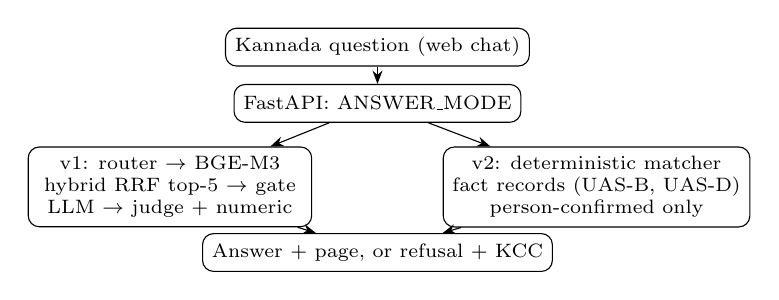
\begin{tikzpicture}[node distance=0.22cm,
  b/.style={draw,rounded corners,align=center,font=\scriptsize,minimum width=3.6cm,minimum height=0.48cm},
  a/.style={-{Stealth}}]
\node[b] (q) {Kannada question (web chat)};
\node[b,below=of q] (m) {FastAPI: ANSWER\_MODE};
\node[b,below left=0.3cm and -1.0cm of m,minimum width=3.6cm] (r) {v1: router $\rightarrow$ BGE-M3\\hybrid RRF top-5 $\rightarrow$ gate\\LLM $\rightarrow$ judge + numeric};
\node[b,below right=0.3cm and -1.0cm of m,minimum width=3.6cm] (f) {v2: deterministic matcher\\fact records (UAS-B, UAS-D)\\person-confirmed only};
\node[b,below=1.4cm of m] (o) {Answer + page, or refusal + KCC};
\draw[a] (q)--(m); \draw[a] (m)--(r); \draw[a] (m)--(f);
\draw[a] (r)--(o); \draw[a] (f)--(o);
\end{tikzpicture}
\caption{Two answer paths share the interface, refusal line and history.}
\label{fig:arch}
\end{figure}

\subsection{Version 1: RAG pipeline}
\textit{Embedding and retrieval.} Chunks of a sugarcane collection are embedded with BGE-M3~\cite{chen2024bgem3}, which gives a dense vector and a learned sparse vector in one pass. The 15 best
chunks by each are fused by reciprocal rank fusion~\cite{cormack2009rrf},
$\mathrm{RRF}(d)=\sum_i 1/(k+r_i(d))$, and the top 5 form the context. For pest and disease
questions, BM25~\cite{robertson2009bm25} and dense ranks are fused instead ($k=60$), because dense vectors confused
pest cards that share remedy wording.

\textit{Router.} An LLM labels the category. The label only tightens the gate; it never
filters retrieval. An early version used it as a hard filter, which made documents of other
categories unreachable when the router erred.

\textit{Abstention gate.} The gate answers only if the dense cosine relevance
$\mathrm{rel}(q)=\cos(\mathbf{q},\mathbf{e}_d)$ of the best chunk is at least $\tau_c$
($0.50$ for pest, disease and fertiliser; $0.35$ otherwise) and, for pest and disease, a
pest or disease name in the question also appears in a retrieved card. RRF scores are never
used here: they depend only on ranks, and the original gate, which used them, let an
unanswerable price question through with score 1.0. The thresholds are uncalibrated: on 18
development questions, relevance of answerable (0.456--0.668) and unanswerable
(0.499--0.597) questions overlapped.

\textit{Generation and checks.} \texttt{gpt-oss-20b} (Groq, temperature 0) answers in Kannada
from the context only. An LLM judge scores faithfulness, and a rule-based checker requires
every (number, unit) pair in the answer to appear in the context. Failing either check
turns the answer into a refusal; every response ends with the KCC number.

\textit{Failures found and fixed.} The router and judge, run on a reasoning model with small
output budgets, returned empty text on 14 of 18 router calls (silently mapped to the
``general'' category) and on several judge calls (scored 0.0). We added larger budgets, one
retry, and an explicit failure state that fails closed. The numeric checker bound numbers to
units inside ordinary words (``10 min is crucial'' read as 10 litres); units now bind only to
the nearest standalone unit word. Table~\ref{tab:defects} lists the safety-relevant defects
found in version~1.

\begin{table}[t]
\centering
\caption{Safety-relevant defects found in version~1}
\label{tab:defects}
\footnotesize
\begin{tabular}{p{2.2cm}p{2.9cm}p{2.4cm}}
\toprule
Defect & Effect & Fix\\
\midrule
Gate read RRF score & Unanswerable price question scored 1.0; never refused & Dense cosine relevance\\
Router label as hard filter & Other categories unreachable when router erred & Filter removed\\
Empty router/judge output & 14/18 router calls silently ``general''; judge 0.0 & Budget, retry, fail closed\\
Judge blind to wrong entity & Wrong-pest dose scored 1.0 & Entity match (v1); v2 design\\
Unit mis-binding & ``10 min'' read as litres & Nearest standalone unit\\
Non-deterministic ties & Different top chunk across runs & Deterministic tie-break\\
\bottomrule
\end{tabular}
\end{table}

\subsection{Version 2: confirmed fact records}
\textit{Motivation.} On held-out questions, version~1 answered a question about an unknown
pest with the early shoot borer doses; the judge scored it 1.0 and the numeric check passed
it, because the answer quoted its retrieved chunk correctly. A check that compares an answer
with its context cannot detect that the context is about the wrong thing.

\textit{Records.} 90 typed records (47 from UAS Bengaluru POP 2025, 43 from UAS Dharwad POP
2020) hold the Kannada text shown to the farmer, the source, the printed page, and verbatim
supporting excerpts. A script checks that each excerpt is on its page and each number in the
text is in the excerpts; this catches copying mistakes, not agronomic ones. Records with
pesticides not registered in India (phorate, metasystox, benomyl) were removed.
Table~\ref{tab:records} shows the records by topic. Other documents (an ICAR advisory, an
IPM package, a Tamil Nadu guide) are used only to cross-check, never as a dose source; where
UAS and a cross-check source differ, the UAS recommendation is given.

\begin{table}[t]
\centering
\caption{Draft fact records by topic}
\label{tab:records}
\footnotesize
\begin{tabular}{lrr|lrr}
\toprule
Topic & B & D & Topic & B & D\\
\midrule
Pests & 12 & 9 & Planting & 2 & 3\\
Varieties & 8 & 3 & Sett treatment & 2 & 2\\
Fertiliser & 5 & 6 & Seed rate & 2 & 1\\
Diseases & 5 & 5 & Irrigation & 1 & 2\\
Ratoon & 4 & 7 & Harvest, soil & 2 & 1\\
Weed control & 4 & 3 & Pesticide safety & 0 & 1\\
\midrule
\multicolumn{6}{l}{Total: 47 UAS Bengaluru (B), 43 UAS Dharwad (D)}\\
\bottomrule
\end{tabular}
\end{table}

\textit{Human confirmation.} A person marks each record CONFIRMED, WRONG or UNSURE against the
printed page. The confirmation stores $h(r)$, the first 16 hex digits of SHA-256 over the
record's farmer-visible fields; a record is usable only if its status is CONFIRMED, $h(r)$
matches the current record, and, if it names a pesticide, its CIB\&RC registration has been
confirmed.

\textit{Matching.} The question is normalised (zero-width characters removed, lower-cased,
spaces collapsed) and matched against pest/disease names, topic keywords, district names and
other-crop words. Longer phrases are matched first and consume their characters, so a short
word inside a longer matched phrase cannot match again. The rules, in order:
\begin{enumerate}
\item names another crop $\Rightarrow$ refuse (out of scope);
\item matches a refused topic such as price $\Rightarrow$ refuse;
\item names a known pest or disease $\Rightarrow$ that subject's records;
\item mentions a pest or disease word but no known name $\Rightarrow$ refuse (unknown pest);
\item matches a topic $\Rightarrow$ that topic's records;
\item otherwise $\Rightarrow$ refuse.
\end{enumerate}
Rule~4 removes the version~1 wrong-pest failure by construction: a dose can only be reached
through the pest's own name. Pest and disease records cannot be reached through a topic
keyword, and symptom words are not treated as names, since that would be diagnosis. Of the
selected records, only usable ones are shown; if none remains, the system refuses. If the
question names a district, only that region's records are shown; otherwise southern and
northern records appear under separate headings and are never merged. The answer is the
stored text, its book and page, a pesticide-safety line when a product is named, and the KCC
number; nothing is generated, so the same question always gets the same answer.

% =========================================================
\section{Results}
\label{sec:results}

\subsection{System and hardware}
Development and evaluation ran on a laptop with an Intel Core i5-1334U and 16\,GB RAM, no
GPU. Software: Python 3.13, FastAPI, Qdrant, MongoDB, FlagEmbedding (BGE-M3), Next.js.
Version~2 needs no GPU and no LLM API.

\subsection{Performance metrics}
Each question is labelled answerable or should-refuse. We report decision accuracy (answerable
answered plus should-refuse refused, over all questions), its two parts, and the number of
\emph{safety failures} (a wrong chemical, dose or unit), which is never averaged away. For
retrieval we report Recall@5, MRR and nDCG@5.

Text-overlap metrics were first checked by scoring each reference against itself.
ROUGE-L gave a mean self-score of 0.625, with 6 of 16 Kannada references at 0.000. chrF
\cite{popovic2015chrf} and BLEU gave 1.0. But in a constructed example
(Table~\ref{tab:overdose}) both score a 10$\times$ overdose far above a correct paraphrase.
We therefore do not use them as quality or safety evidence.

\begin{table}[t]
\centering
\caption{Scores against ``carbendazim 50 WP at 1 g/L, dip setts 15 min'' (constructed)}
\label{tab:overdose}
\begin{tabular}{lrr}
\toprule
Answer & chrF & BLEU\\
\midrule
Same text, 10 g/L (10$\times$ overdose) & 96.7 & 83.9\\
Correct paraphrase, 1 g/L & 62.5 & 30.9\\
\bottomrule
\end{tabular}
\end{table}

\subsection{Results}
\textit{Retrieval (version 1).} Table~\ref{tab:retrieval} compares retrieval settings on 15
answerable development questions over the original 43-chunk collection. Hybrid retrieval
found the relevant chunk in the top 5 for every question, while dense-only ranked it first
more often (higher MRR). With recall at ceiling, a cross-encoder reranker had little to fix
and added about 30\,s per query on CPU, so it is off. BM25+dense was used for pest and
disease questions, where exact names matter. The relevant-chunk labels were assigned during
development, with AI assistance, not by an expert, so these figures are indicative.

\begin{table}[t]
\centering
\caption{Retrieval on 15 answerable development questions (mean)}
\label{tab:retrieval}
\footnotesize
\begin{tabular}{lccc}
\toprule
Setting & Recall@5 & MRR & nDCG@5\\
\midrule
Dense only & 0.933 & 0.848 & 0.862\\
Hybrid (dense + sparse, RRF) & 1.000 & 0.749 & 0.817\\
BM25 + dense & 0.933 & 0.819 & 0.842\\
\bottomrule
\end{tabular}
\end{table}

\textit{Abstention gate (version 1).} On 18 development questions, a question about ``black
beetle'', a pest not in the collection, retrieved the termite card at relevance 0.597, above
two answerable questions, and the model gave the termite dose; the faithfulness judge rated
the answer 1.0. Relevance therefore cannot separate ``similar but wrong'' from ``correct'',
which is why the entity-match rule was added and why we did not tune thresholds on this data.

\textit{Held-out (version 1).} On 40 held-out questions (24 answerable, 16 should-refuse)
with the code frozen, version~1 made 29 correct decisions: 14/16 should-refuse questions
refused and 15/24 answerable answered (Table~\ref{tab:heldout}). Of the 9 refused answerable
questions, 5 had expected answers from a document outside the collection. The one safety
failure was the wrong-pest answer described above: the entity match was satisfied by the
generic word for ``worm'', which is part of the early shoot borer's Kannada name.

\textit{No-retrieval baseline.} The same model with no documents refused only 4 of the 16
should-refuse questions; 7 of its answers contained a dose-like number and unit (categories
assigned by reading the answers, with AI assistance; indicative).

\begin{table}[t]
\centering
\caption{Held-out evaluation (decisions correct / total)}
\label{tab:heldout}
\begin{tabular}{lccc}
\toprule
System & Refuse & Answer & Safety failures\\
\midrule
LLM, no retrieval & 4/16 & -- & 7 dose-like$^{*}$\\
Version 1 (RAG) & 14/16 & 15/24 & 1\\
Version 2, pilot 1 (15 records) & 10/10 & 8/10 & 0\\
Version 2, pilot 2 (50 records) & 3/3 & 6/7 & 0\\
\bottomrule
\end{tabular}\\[2pt]
{\footnotesize $^{*}$Answers to should-refuse questions containing a number and unit;
correctness not assessed.}
\end{table}

\textit{Version 2: review.} A team member reviewed 52 of the 90 records against the printed
pages in three rounds; 50 are confirmed and usable. Each ``registered'' answer was
cross-checked in the CIB\&RC lists: chlorpyrifos (early shoot borer; termite soil
treatment), chlorantraniliprole 0.4\% GR, fipronil 0.3\% GR and atrazine 50\% WP have
sugarcane entries, but carbendazim, recommended in both books for sett treatment, has none
(only sugar beet). Both sett-treatment records were held as UNSURE and are refused: a dose
printed in an official book but not supported by the current registration list.

\textit{Version 2: pilot 1} (15 records). On 20 new questions written by a team member with
AI assistance (so expected answers were checked against the page excerpts rather than
trusted), version~2 made 18 correct decisions with no wrong dose. All 10 should-refuse
questions were refused, including two pesticide-dose questions (no pesticide record was
confirmed yet). The 2 errors were answerable questions refused because their wording
(``seed cane or buds'', ``how to choose setts'') was not in the keyword lists; the lists
were not changed before reporting. In two answered questions the writer's expected answer
differed from the book, and the system's answer matched the verbatim page excerpt.

\textit{Version 2: pilot 2} (50 records). Ten questions on the newly confirmed pest, weed
and striga topics gave 9 correct decisions: the 3 unknown pests (fall armyworm, whitefly,
nematode) were refused, and 6 of 7 answerable questions were answered from the right records.
The miss asked about \emph{stem} borer while expecting the \emph{early shoot} borer answer;
stem borer has no record, so the system refused it, which is the intended behaviour. This
writer had seen the records, so the pilot is less independent.

Across both pilots, 27 of 30 decisions were correct and no answer gave a wrong dose. By the
rule of three~\cite{hanley1983zero}, zero failures in $n$ questions bounds the failure rate
below about $3/n$, here 10\%: the pilots show that the design works as intended, not that it
is safe in general.

The 10 should-refuse questions covered an unlisted pest (armyworm), a disease without a
confirmed record (brown spot), two other crops (paddy, maize), two price questions,
weather, a machinery subsidy, and two pesticide-dose questions (early shoot borer,
termites). After the run, the two missing phrases were added to the keyword lists, with a
test that the new seed-rate phrase does not hide the internode borer's Kannada name, which
shares the word for ``node''; a re-run then answered all 20 correctly, but this is not a
held-out result. Table~\ref{tab:examples} shows four real responses.

\begin{table}[t]
\centering
\caption{Real version 2 responses (English glosses of the Kannada output)}
\label{tab:examples}
\footnotesize
\begin{tabular}{p{2.5cm}p{5.2cm}}
\toprule
Question & Response\\
\midrule
NPK per acre for sugarcane in Mandya? & UAS Bengaluru 2025 (South): N 100\,kg, P 40\,kg, K 50\,kg per acre (p.\,166); 10\% N at planting, 20\% at 45 days, 30\% at 75, 40\% at 105 (p.\,167). + KCC line\\
\addlinespace
Black beetle on my cane; what to spray? & No verified information on this pest; a wrong pesticide is dangerous, so we will not guess. + KCC line\\
\addlinespace
Fertiliser for tomato? & I only answer these sugarcane topics: varieties, planting season, seed rate, \dots{} + KCC line\\
\addlinespace
Current sugarcane price? & No expert-verified information on this yet. + KCC line\\
\bottomrule
\end{tabular}
\end{table}

\subsection{Discussion}
\textit{Faithful is not correct.} Both version~1 checks compare the answer with the retrieved
text. When retrieval returns the nearest pest's card, a faithful answer is a wrong answer, so
neither check can catch it. RAG evaluation that scores faithfulness alone~\cite{es2023ragas}
would rate this failure as a success.

\textit{Similarity is not a refusal signal.} As in selective QA~\cite{kamath2020selective},
the system's own scores were poorly calibrated for abstaining: relevance for unanswerable
questions overlapped that of answerable ones. Version~2 decides by whether a confirmed record
exists for a named subject, not by a score.

\textit{The cost is coverage.} Version~2 refuses anything outside its confirmed records and
keyword lists. In this domain we consider that the right trade-off: a refusal costs the farmer
a phone call to the KCC, a wrong dose can cost the crop. Coverage grows by reviewing more
records and adding wordings, both of which are checked by tests and by a person.

\textit{Evaluate what matters.} Reporting decision accuracy together with a separate count of
wrong doses made the version~1 safety failure visible; an average text-similarity score would
have hidden it (Table~\ref{tab:overdose}).

% =========================================================
\section{Conclusion}
\textbf{Problem:} a Kannada assistant for sugarcane farmers must never give a wrong
chemical or dose. \textbf{Solution:} we built a RAG pipeline, found and fixed the failures
that silently reduced its safety, measured it with metrics that count correct refusals, and
replaced its answer path with person-confirmed fact records and deterministic matching.
\textbf{Achieved:} evidence that common text metrics fail on Kannada advisory answers, a
held-out evaluation of 29/40 with one wrong-pest failure that both answer checks missed, and
a design that removes that failure by construction. \textbf{Drawbacks:} version~2 covers only
confirmed records from two sugarcane chapters; questions in unexpected wording are refused;
review so far is by the team, not an expert; the pilot is small; and the held-out questions
were written with partial AI assistance, so results are indicative.

\textbf{Future work.} (1) Complete confirmation of the remaining 40 records, including 23
that name a chemical, each with its current CIB\&RC registration checked by a person, and a
registration source for carbendazim. (2) Expand the evaluation set with real farmer
questions: Kisan Call Centre query logs for Karnataka sugarcane and transcriptions of real
Kannada calls or village extension workers' conversations, labelled by experts. (3) Hybrid
middle grounds: we have implemented an optional canonicaliser in which an LLM is used solely
for intent extraction, constrained by a JSON-schema enumeration to the 40 topic labels that
lead to no pest or disease record, consulted only when the keyword matcher finds nothing,
and validated strictly, so it can never reach a dose; 34 tests with a simulated model pin
these properties. In one live probe (gpt-oss-20b, structured output) on 19
developer-written questions that the keyword lists miss, it chose the right topic for 9 of
10 and answered ``none'' for all 9 that must be refused (rats, wild boar, symptoms, loans);
all replies were valid. It remains to evaluate it on real farmer questions.

\bibliographystyle{IEEEtran}
\bibliography{references}

\end{document}
